\documentclass[10pt,twocolumn]{witseiepaper}
\usepackage{KJN}
\usepackage{url}

\usepackage{float}
\usepackage{graphicx}
\usepackage{tikz}
\usepackage{pgfplots}
\usepackage{circuitikz}
\usepackage{multirow}
\usepackage{tabto}
\usepackage[bottom]{footmisc}
\usetikzlibrary{shapes.geometric, arrows}


\ifpdf
\pdfinfo{
	/Title (INSTRUCTIONS AND STYLE GUIDELINES FOR THE PREPARATION OF FINAL YEAR LABORATORY PROJECT PAPERS : 2005 VERSION)
	/Author (Ken J Nixon)
	/CreationDate (D:200309251200)
	/ModDate (D:200510121530)
	/Subject (ELEN417/455 Paper Format, 2005)
	/Keywords (ELEN417, ELEN455, paper, instructions, style guidelines, laboratory project)
}
\fi


%%%%%%%%%%%%%%%%%%%%%%%%%%%%%%%%%%%%%%%%%%%%%%%%%%%%%%%%%%%%%%%%%%%%%%%%%%
\begin{document}
	
	
	\title{First Prototype Design and Execution of a Smart Home Power Management System\\ 2016/04/11}
	
	\author{Ari Croock - 718005\\Kanaka Babshet - 678851\\Alice Yang - 597609\\Daniel Weinberg - 547937\\\\ELEN4009 - Software Engineering}
	\thanks{School of Electrical \& Information Engineering, University of the
		Witwatersrand, Johannesburg}
	%%%%%%%%%%%%%%%%%%%%%%%%%%%%%%%%%%%%%%%%%%%%%%%%%%%%%%%%%%%%%%%%%%%%%%%%%%%%%%%
	%
	\abstract{This paper details the design and implementation of the first prototype of a smart home power management system. The final project submission is composed of an application which can add a household device, and control its state, as well as a compilation of all the documentation written in the process of designing this application. A critical analysis of the issues experienced during the design, implementation, and testing, has been provided. All constraints and specifications are successfully met, and additional improvements (as stated herein) can still be made in the future.}
	
	\keywords{Design, Smart Home, Power Management, Internet of Things}
	
	\maketitle
	\thispagestyle{empty}\pagestyle{empty}
	
	
	%%%%%%%%%%%%%%%%%%%%%%%%%%%%%%%%%%%%%%%%%%%%%%%%%%%%%%%%%%%%%%%%%%%%%%%%%%%%%%%
	%
	\section{INTRODUCTION}
	
	A smart home power management system allows users to control and supervise various electrical devices within the household in order to manage the overall power consumption. The system also automatically manages various devices without human interaction depending on the settings enabled in advance by the system user.
	This interaction and status display is done via a webpage accessible to all predefined household users. 
	
	The aim of this project is to design the complete aforementioned system and implement some aspect of the system which is defined as the first prototype. The prototype implemented is made up of a scrollable webpage, with a page header and tabs, the addition and removal of a device, with corresponding specifications, viewing the devices connected, and toggling between the states of devices. 
	
	Section 2 details the software requirement specification, and is followed by section 3 which contains an extensive design document split into the relevant front and back end sections. Section 4 introduces the sprint planning and illustrates the work breakdown over the time designated for this project, while section 5 provides a sprint retrospective. Section 6...
	\section{SOFTWARE REQUIREMENT SPECIFICATION}
	
	\subsection{Purpose}
	This section details the system requirements specification (SRS) for the Smart Home Power Management System. The system design documentation will be developed from this information.\\
	\newline 
	With the rapidly growing interest in new Internet of Things (IoT) technologies, networks consisting of these devices will become increasingly difficult to manage and control. Additionally, power consumption and monitoring will become a greater concern, especially in emerging markets such as South Africa.\\
	\newline 
	This project aims to provide a flexible software system which is able to remotely control and monitor IoT devices, as well as perform detailed power consumption diagnostics.
	
	\subsection{Project Scope}
	The project is a system that will allow for remote control, monitoring and automation of IoT devices on a Local Area Network (LAN). A client-server architecture will be used since this allows a back-end server to continuously manage devices while allowing for a client to connect on-demand. The front-end will initially be implemented as a web page for simplicity and compatibility with many existing devices (such as cellphones and personal computers). \\
	\newline 
	The back-end provides functionality to control and monitor devices, and to log device power consumption. Additionally, the back-end will contain the web server used for interfacing with users. \\
	\newline
	The front-end will consist of a web-based user interface which will provide secure access to a device dashboard. The dashboard will provide remote control and configuration of devices, as well as access to power consumption data. Addition and removal of IoT devices will also be performed through the dashboard. 
	
	\subsection{Project Overview}
	
	Figure~\ref{fig:dfd} shows a data flow diagram of the system. Data collected from IoT devices is stored in a database and used to control other devices as defined by the user. A web interface allows the user to configure devices and to view the stored data.
	\begin{figure}[!htb]
		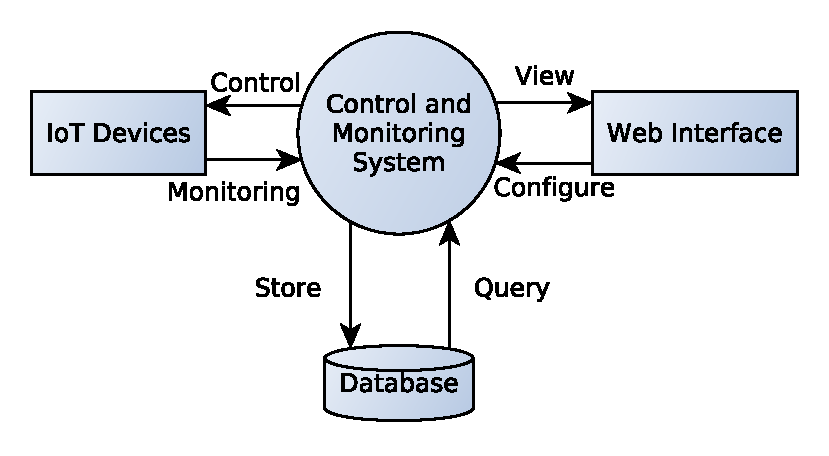
\includegraphics[width=\columnwidth]{data-flow-1}
		\caption{Data flow diagram (DFD) of the system. All data flows are bidirectional}
		\label{fig:dfd}
	\end{figure}
	
	\subsubsection{Assumptions:}
	\begin{itemize}
		\item All of the IoT devices will be connected to the same LAN
		\item Only a small number of simultaneous users and devices will be connected at once
	\end{itemize}
	\subsubsection{Constraints:}
	\begin{itemize}
		\item The user interface must be accessible through a web browser
		\item All devices in the system require wireless connectivity
	\end{itemize}
	
	\subsubsection{User Classes and Characteristics:}
	\begin{itemize}
		\item Basic users who can configure basic devices and view power usage statistics
		\item Advanced users who can configure custom devices and export power usage statistics for further processing
	\end{itemize}
	
	\subsubsection{Operating Environment:}
	The following technologies will be used to implement the system:
	\begin{itemize}
		\item Django Web Framework (Python 3.5.1)
		\item PostgreSQL Database Management System (DBMS)
		\item Docker 1.8.2
	\end{itemize}
	Assuming that few users and devices will be connected to the system simultaneously (such as in a typical household), the system requirements are fairly relaxed:
	\begin{itemize}
		\item any modern Microsoft Windows or GNU/Linux system that supports the technologies used
		\item a connection to the LAN, such as Ethernet or WiFi
		\item low-cost hardware such as a Raspberry Pi
	\end{itemize}
	However, depending on the system configuration, an external storage solution may be needed for storing a large amount of power usage data.
	
	%3 tier has better security because 2 tier the client is allowed access and communication with 
	
	\subsubsection{Software Development Life-cycle:}
	The system will be developed using an Agile software development methodology. In particular, the popular SCRUM framework will be used so that the system's requirements and design details can change quickly if need be. 
	
	\subsection{System Features}
	The smart home power management system is made up of various features which enhance the usability of the product, along with some additional features which simplify all related functionality.
	\subsubsection{System Feature 1 - Remote On/Off Switching: } 
	Switch any of your selected appliances on or off from any personal device connected to the home network. 
	\newline
	\textbf{Description:}
	The user can control the power status of various appliances in the household. The appliances are connected independently, for which reason, multiple appliances can be controlled through the same interface, simultaneously. 
	\newline
	\textbf{Stimulus/Response Sequences:}
	The user has to select the "Power Remote" tab on the home page to display the on and off options corresponding to each connection. 
	%\subsubsection{Functional Requirements}
	
	\subsubsection{System Feature 2 - User Configurable Triggers:} 
	Personalise various situations which will trigger an action.
	\newline
	\textbf{Trigger 1 - Motion Detection:}
	Set appliances to switch on or off depending on surrounding motion. 
	\newline
	\textit{Description:}
	The user can control whether specific appliances must be configured with motion detection or not. For example, if motion detection is set for a certain set of lights, they will detect movement in the surrounding area and switch on, or switch off when there is no motion detected for a set period of time. If the user does not want an appliance or set of lights to be triggered by motion, the respective switch is "off" on the webpage. 
	\newline
	\textit{Stimulus/Response Sequences:}	
	The user has to select the "Triggers" tab from the home page, and thereafter select the "Motion Detection" tab at the top left of the newly loaded page to display the corresponding settings. Figure \ref{Trigger_Tab} in Section 4 below illustrates this page. 
	\newline
	\textbf{Trigger 2 - Temperature Detection:}
	Set appliance statuses to vary depending on the surrounding temperature.
	\newline
	\textit{Description:}
	The user can control whether specific appliances must be configured with heat triggers or not. For example, if temperature detection is set for a specific appliance, it will detect a certain temperature in the surrounding area and switch on, switch off, or maintain state if it is too hot, too cold, or within the correct temperature range depending on the user choices. If the user does not want an appliance or set of lights to be triggered by the ambient temperature, the respective switch is "off" on the webpage. 
	\newline
	\textit{Stimulus/Response Sequences:}	
	The user has to select the "Triggers" tab from the home page and thereafter select the "Temperature Detection" tab at the top of the newly loaded page, (second from the left), to display the corresponding settings.
	\newline
	\textbf{Trigger 3 - Light Detection:}
	Set appliance statuses to vary depending on the surrounding light.
	\newline
	\textit{Description:}
	The user can control whether specific appliances must be configured with light triggers or not. For example, if light detection is set for a specific appliance, it will detect a certain ambient light level in the surrounding area and correspondingly vary, or maintain state depending on the user choices. If the user does not want an appliance or set of lights to be triggered by the ambient light levels, the respective switch is "off" on the webpage. 
	\newline
	\textit{Stimulus/Response Sequences:}
	The user has to select the "Triggers" tab from the home page and thereafter select the "Light Detection" tab at the top of the newly loaded page, (third from the left), to display the corresponding settings.
	\newline
	\textbf{Trigger 4 - Time Scheduling:}
	Select and adjust times for the different appliances to be on, off, or running on defined settings. 
	\newline
	\textit{Description:}
	The user can activate time scheduling for each device/set of lights independently connected to the smart home power management system. For example, the user can set the geysers to switch on from 6 am to 8 am and from 7 pm to 9 pm everyday. Note that the selection of time scheduling for appliances does not affect the user's ability to manually control the power via the system, or directly in person. 
	\newline
	\textit{Stimulus/Response Sequences:}
	The user has to select the "Triggers" tab from the home page and thereafter select the "Time Scheduling" tab at the top right of the newly loaded page to display the corresponding settings.
	\subsubsection{System Feature 3 - Power Consumption Monitoring:}
	Monitor the power consumption by various appliances and sets of lights in the household. 
	\newline
	\textbf{Description:}
	Given that this system is based on power management, the user can easily view detailed layouts of the total household power consumption data and analytics. The user will be able to view graphical statistics of the power consumption over the course of the day, as well as detailed statistics over a longer period of time (previous month, or year). This allows the user to compare the household power consumption with that of the usage if this system was not implemented. 
	\newline
	\textbf{Stimulus/Response Sequences:}
	The webpage automatically starts on the "Home Status" tab upon loading. The user can view this page for a daily consumption summary, and can then click on the "Consumption Monitoring" tab seen on the left of the same page to view these analytics in greater detail, over a longer period of time.
	\subsubsection{System Feature 4 - Energy Source Management:}
	Control and manage the different energy sources in the household such as varying the usage between electricity and solar power.
	\newline 
	\textbf{Description:}
	This system encourages the use of alternative, renewable energy sources. If the user has catered for these facilities, the system allows additional power volume management through the energy source management configuration. 
	\newline
	\textbf{Stimulus/Response Sequences:}
	The user has to select the "Energy Source Management" tab on the left of the homepage to be directed to this page. 
	\subsubsection{System Feature 6 - User Configurable Alerts:} 
	Choose which events should result in an immediate alert/notification on your system.
	\newline 
	\textbf{Description:}
	Along with all the personalised settings configured on the system, the user is able to define situations in which alerts appear on the system and possibly directly to the user's smart device. 
	\newline
	\textbf{Stimulus/Response Sequences:}
	The user has to select the "Alerts" tab on the left of the homepage to then configure these settings.
	\subsubsection{System Feature 7 - User Configurable Webpage Settings} 
	Define webpage settings in order to enhance the power management system experience.
	\newline
	\textbf{Description:}
	The user can add or remove devices to be controlled by the smart home power management system, alter the webpage appearance, manage users on the network, and edit security settings. 
	\newline
	\textbf{Stimulus/Response Sequences:}
	The user must click on the "Settings" link to the right of the title on the home page to be able to configure all the required settings.
	
	\subsection{External Interface Requirements}
	The external interface is the interface which allows the user to interact with the system through a hardware device using software. The external interfaces consists of a user interface, hardware interface, software interface and communication interface. 
	
	\subsubsection{User Interface - GUI:}
	The user interface is how the user will interact with the system. The requirements for the design of user interface must be simple and easy to navigate. A simple format of representing all the devices connected to the Smart Home Power Management System is to display the features available for all devices on a dashboard. This can been seen in Figure \ref{Home_Dashboard}.
	
	Figure \ref{Trigger_Tab} is a simple illustration of the interface between the user the light detection triggers on the system. The layout of the tab is further divided to clearly illustrate the sub-systems which the user has access to. As seen from the figure, the switches on the triggers tab are designed in a graphical format that is simple for users to use.  
	
	Figure \ref{Settings} is the settings page, in which it designed for the user to navigate through each sub-system. The \textit{Add/Remove Device} feature is an important feature, as it is expected that the client may have to add or remove devices for future use. The settings page is set up similarly to the home page on the trigger tab, as user's  familiarity to the website is of importance.
	
	\begin{itemize}
		\item Home Page Dashboard
		\begin{figure}[!h]
			\centering
			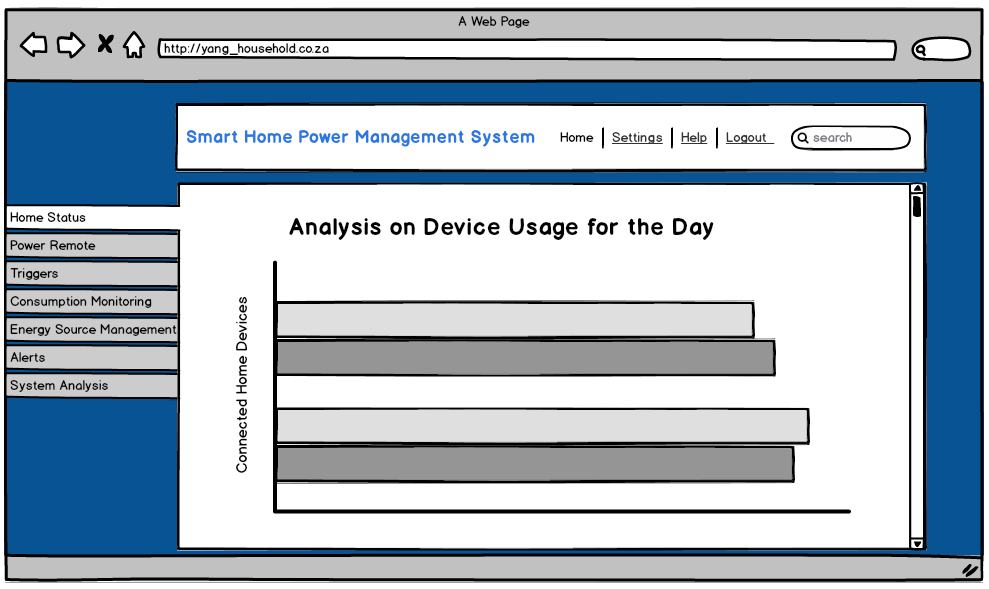
\includegraphics[width=\linewidth]{Home_Page.png}
			\caption{Figure illustrating the home page the user will see once they have logged on to access the system.}
			\label{Home_Dashboard}
		\end{figure}
		\pagebreak
		\item Trigger Tab on Dashboard
		\begin{figure}[!h]
			\centering
			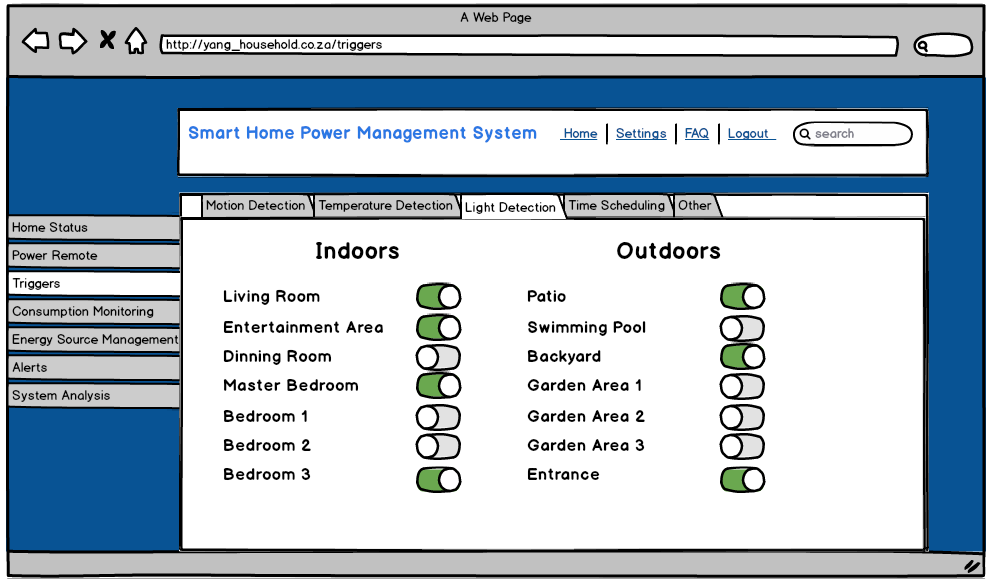
\includegraphics[width=\linewidth]{Trigger_Tab.png}
			\caption{Figure illustrating the triggers tab, to allow users to control switching of sensors in their home through the system.}
			\label{Trigger_Tab}
		\end{figure}
		\item Settings Page
		\begin{figure}[!h]
			\centering
			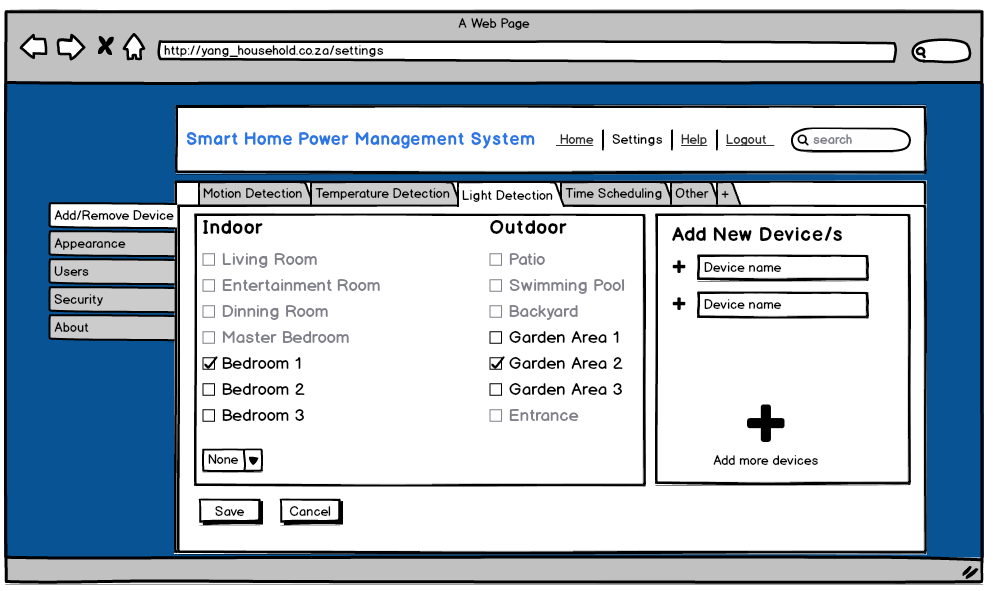
\includegraphics[width=\linewidth]{Settings.png}
			\caption{Figure illustrating the settings page.}
			\label{Settings}
		\end{figure}
	\end{itemize}
	
	\subsubsection{Hardware Interface:}
	The user interface is implemented on a web based platform that is accessible through a browser. The hardware required to access the system can be either of the listed devices found in the list below:
	
	\begin{itemize}
		\item Large Desktops (1200 -  pixels)
		\item Medium Desktops (992 - 1199 pixels)
		\item Small Devices (768 - 991 pixels)
		\item Extra Small Devices (max 767 pixels)
	\end{itemize}
	
	\subsubsection{Communication Interface:}
	The Smart Home Power Management System is a web-based application that requires a internet connection for the communication between the hardware devices, system and IoT devices. The main connection between the system and the IoT devices is through the user's home wireless connect (WiFi). For the hardware device to communicate with the system any type of internet connection will do.
	
	\subsection{Other Non-Functional Requirements}
	
	\subsubsection{Performance Requirements:}
	The smart home power system is an application and system that is designed for efficiency. This means that the application as well as the connecting household components need to respond quickly and in real time. 
	\\\\
	The application will most likely undergo several updates and changes for the user's benefit. The system is required to update on user command. Updates will include further improvements to the application as well as fixes for issues that arise in operation.
	
	\subsubsection{Safety Requirements:} 
	The application as well as the system components need to take certain safety concerns into account. 
	\\\\
	Due to the fact that the application is essentially controlling most of a home's appliances and electricity usage, it is important that it monitors everything it is controlling to prevent problems that may arise. The application needs to ensure that any device connected in the system does not reach a dangerous level of usage. In this case, the application should either switch off the device in question or notify the user that something is not functioning correctly and needs to be addressed. 
	
	\subsubsection{Security Requirements:}
	Due to the fact that the system controls a user's home, it therefore requires security considerations to be taken into account.
	\\\\
	The system needs to ensure that only the user has access to the application to prevent external parties gaining control of the connected components within a house. This can be done with a signup, login and authentication process. 
	The components within the house that the application connects with, need to be protected from external parties and therefore they must be explicitly authenticated. 
	
	\subsubsection{Software Quality Attributes:}
	The application is web based and needs to be user friendly. The functioning of the application needs to be simple so that no additional documentation or prior knowledge or experience is required. 
	
	\section{DESIGN DOCUMENT}
	
	The purpose of this section is to provide details regarding the software development of the project. 
	
	\subsection{Scope}
	The scope of the project is for a basic prototype of the proposed power management system. The focus of the system is to manage connected devices and their corresponding power usage data. 
	
	The scope of this prototype, however, is limited to the management and analytics portion of the complete system, not the inter-device communication aspect. 
	
	\begin{center}
		\textbf{I. FRONT-END}
	\end{center}
	
	\subsection{Overview}
	The front-end of the power home management system is an integral component of the system as a whole. Without the presence of the front-end, the back-end becomes essentially irrelevant. The front-end allows the user to interact with the smart home system through a web-page platform. Within the front-end are graphical and functional features that makes the connected devices easily controlled. The front-end consists of a login page, an administration page, a settings page, a device details page, both individual and collective, as well as a dashboard page containing system and device diagnostics.
	
	\subsubsection{Purpose}
	The purpose of the front-end is to provide a user friendly graphical user interface which allows the user to interact with the smart home power management system. It provides a means of communication between the front-end and the back-end of the system in order to display the relevant information or changes to the user. In addition it allows the user to control the devices remotely through the platform at any location.
	
	\subsubsection{Scope}
	The implementation of the front-end is for a smart home power management system which monitors the usage and power consumption. It therefore allows user the ability to alter power usage as well as configure alerts and manage the settings of the front-end. The front-end also allows the user to initiate remote triggering of connected devices such as lights and kitchen appliances. It is also designed to display the outcomes of triggering motion detectors and temperature sensors.
	
	\subsubsection{Definitions, Acronyms and Abbreviations}
	\begin{itemize}
		\item \textbf{CSS} - Cascading Style Sheets which is a stylesheet language that sets up the appearance of the HTML \cite{CSS}.
		\item \textbf{HTML} - Hypertext Markup Language which is used to generate web pages and its objects form the basis of all websites \cite{HTML}.
		\item \textbf{Django} - A framework used to compile and render the HTML pages.
		\item \textbf{Bootstrap} - provides a html and css template for web development
		\item \textbf{Javascript} - A high level and dynamic programming language that is used with HTML and the web \cite{Javascript}.
	\end{itemize}
	
	\subsection{Use Cases}
	The use cases for the front-end are as given in the tables below. 
	\begin{table}[H]
		\centering
		\caption{Table illustrating the details of the use case for trigger switches}
		\label{trigger_switching_use_case}
		\begin{tabular}{| p{22mm} | p{50mm} |}
			\hline
			\textbf{Use Case} & \textbf{Trigger Switches}\\
			\hline
			Description & The goal of the trigger switching is to allow the users to manually control the connected devices' state through a web-page platform.\\
			\hline
			Actors & Users within a household \\
			\hline
			System Under Design & Web-page Platform for trigger switching\\
			\hline
			Preconditions & The user has successfully passed the authentication process via the login system.\\
			\hline
			Assumptions & It is assumed that the user has a basic understanding of how to access a web-page platform using technological devices.\\
			\hline
			Non-Functional Requirements & The switches are required to be instantaneously responsive when triggered. In addition the triggers must be able to tolerate system malfunctions. .\\
			\hline
			Frequency & The usage frequency of the trigger switches are on a hourly to daily bases \\
			\hline
			Priority & It is of priority, as it is the most accessed functionality in the Smart Home Power Management system. It is also of importance since the functionality allows the user to override the time scheduling settings.\\
			\hline
		\end{tabular}
	\end{table}
	%\pagebreak
	\begin{table}[H]
		\centering
		\caption{Table illustrating the details of the use case for the addition and removal of household devices}
		\label{addition_removal_use_case}
		\begin{tabular}{| p{22mm} | p{50mm} |}
			\hline
			\textbf{Use Case} & \textbf{Addition and Removal of Devices}\\
			\hline
			Description & The purpose of the feature is to enable the user to add and remove devices on the system. \\
			\hline
			Actors & Administration user \\
			\hline
			System Under Design & Addition and Removal web-page platform \\
			\hline
			Preconditions & The user has passed the authentication procedure and they have administration rights. \\
			\hline
			Typical Flow of Events & 1. User logins into the system\\
			& 2. Accesses the administration web-page \\
			& 3. Selects the \textit{Add Device} option \\
			& 4. Provides device details in the allocated input boxes \\
			& 5. Once satisfied with the details of the devices, then select the \textit{save} button to save. \\
			\hline
			Assumptions & There is at least one allocated administration user in the household.\\
			\hline
			Non-Functional Requirements & The addition and removal of the devices in the system is expected to instant, to prevent any confusion to any of the users.\\
			\hline
			Frequency & The frequency usage of the addition and removal feature is low, since the devices will be added during the installation of the systems. If there are any device removals, this will only occur on occasion when the device/s are defective.\\
			\hline
			Priority & This is a high priority feature in the system, as this system is reliant on the ability of the administration user to add and remove devices. Without this feature, the system becomes redundant.\\
			\hline
		\end{tabular}
	\end{table}
	%\pagebreak
	\begin{table}[H]
		\centering
		\caption{Table illustrating the details of the use case for the authentication procedure}
		\label{authentication_use_case}
		\begin{tabular}{| p{22mm} | p{50mm} |}
			\hline
			\textbf{Use Case} & \textbf{Authentication Procedure} \\
			\hline
			Description & The aim of the authentication procedure is to ensure security on the system which results in preventing unwanted user access. \\
			\hline
			Actors & User that wishes to access the system \\
			\hline
			System Under Design & Authentication procedure\\
			\hline
			Preconditions & The user must have previously created an account on the system. \\
			\hline
			Typical Flow of Events & 1. User accesses login page. \\
			& 2. User provides valid username in the allocated input box.\\
			& 3. User provides valid password in the allocated password input box. \\
			& 4. Select \textit{Login} button to submit details for validation.\\
			\hline
			Assumptions & It is assumed that the user has an already existing account. In addition it is assumed that once the user has logged into their account, they remain logged in.\\
			\hline
			Non-Functional Requirements & The procedure is required to hide the password provided by the user and allow immediate access to the user once the provided information is verified.\\
			\hline
			Frequency & Moderate usage due to the assumption that once the user has logged in, the user remains logged unless they are accessing the system from a new mobile or desktop device.\\
			\hline
			Priority & The authentication procedure has high priority, due to the fact that the user is required to log in to access the system. This is important in terms of security, which prevents unwanted users from accessing it.\\
			\hline
		\end{tabular}
	\end{table}
	%\pagebreak
	\begin{table}[H]
		\centering
		\caption{Table illustrating the use case of settings procedure}
		\label{settings_use_case}
		\begin{tabular}{| p{22mm} | p{50mm} |}
			\hline
			\textbf{Use Case} & \textbf{Settings Procedure} \\
			\hline 
			Description & The focus of the settings page is to enable the user to alter both the settings of the connected devices as well as the appearance of the web-page to the user's needs.\\
			\hline
			Actors & Household users \\
			\hline
			System Under Design & Settings Procedure \\
			\hline
			Preconditions & The user is required to have passed the authentication procedure by the logging into the system.\\
			\hline
			Typical Flow of Events & 1. Accessing the settings page \\
			& 2. Selecting either the settings for the connected devices or the appearance of the web-page. \\
			& 3. The settings for the connected devices is performed by selecting the desired device that the user wishes to alter. \\
			& 4. The appearance settings is opened by selecting the \textit{Appearance} tab, in which this takes the user to the web-page that enables them to alter the settings to their customized needs.\\
			& 5. For both the settings the user is required to select the \textit{save} button to ensure that the alterations made are saved.\\
			\hline
			Assumptions & There are default settings implemented for each device during the system installation.\\
			\hline
			Non-Functional Requirements & The settings page is required to be easily accessible and understood by the user to ensure that it is user friendly.\\
			\hline
			Frequency & Moderate usage, since the settings will be performed during installation. It will only be accessed by the user should the user wish to adjust the settings due to changes done in the system. \\
			\hline
			Priorities & High priority, since this establishes the operations of each device. This includes timing, automating devices and power monitoring.\\
			\hline
		\end{tabular}
	\end{table}
	%\pagebreak
	\begin{table}[H]
		\centering
		\caption{Table illustrating the use case of the device details page}
		\label{device_details_use_case}
		\begin{tabular}{| p{22mm} | p{50mm} |}
			\hline
			\textbf{Use Case} & \textbf{Device Details Page}\\
			\hline
			Description & The goal of the device details page is to inform the user of the details of each individual connected devices. In addition it displays the power consumption of each connected devices, as well as the total power consumption in a graphical format.\\
			\hline
			System Under Design & Device Details Page \\
			\hline
			Preconditions & The devices are required to be connected to the system and the user must have passed the authentication procedure to have access the device details. \\
			\hline
			Assumptions & It is assumed that the devices are connected to the system, and that the user has an account. \\
			\hline
			Non-Functional Requirements & It is required to instantly display the device details in a method that is easily understood by the user.\\
			\hline
			Frequency & High usage, since the main reason for the Smart Home system is to manage the power consumption and save, the details device page is predicted to be accessed often to enable the user to analyse the power consumption in their home.\\
			\hline
			Priority & High priority, because this is a crucial component of the system, which entails the details of the each device and its power consumption.\\
			\hline
		\end{tabular}
	\end{table}
	%\pagebreak
	
	\subsection{Design Overview}
	The Design Overview is a section in which it illustrates the architecture of the front-end implementation in the system. It further places it into context with external systems in which is enables the reader of this document to understand the overall details of the front-end design.
	
	\subsubsection{Overall Architecture}
	\begin{figure}[!htb]
		\centering
		\label{system_architecture}
		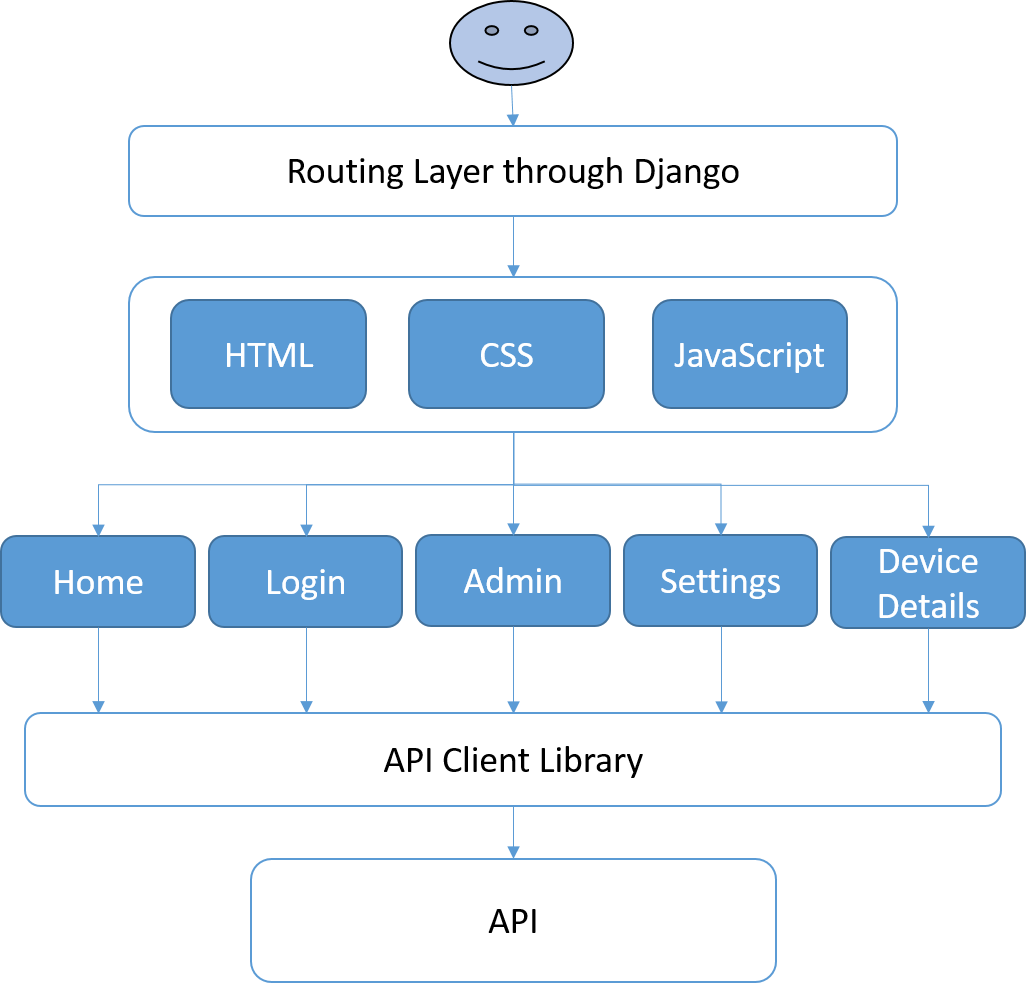
\includegraphics[width=0.9\linewidth]{System_Architecture}
		\caption{Figure showing the front-end system architecture}
	\end{figure}
	
	\subsubsection{System Interfaces}
	An interface is a shared boundary across which two separate components exchange information
	\newline
	\textbf{External User Interface Requirements: }
	\begin{enumerate}
		\item \textit{User interfaces}: The user interface enables the user to interact with they system using a graphical user interface (GUI). This can occur without any knowledge of the back-end functionality. The GUI is in the form of a web page which provides a platform for the user to communicate with multiple connected devices. The interface requires a digital device such as a mobile or desktop device which consists of a screen and keyboard. The GUI is designed in such a way as to create an easily navigable display to ensure it is user friendly.
		\item \textit{Software Interfaces}: The front-end is required to interact with the management system in order to obtain data from the database. This is done by using the supplied Django library namely, \textit{django.shortcuts}, in which the functions \texttt{render()} and \texttt{get\_object\_or\_404()} are used to link the back-end with the front-end HTML. 
		\item \textit{Communication Interfaces}: The communication between the management system back-end and the front-end is performed using JavaScript. The connection enables the user to interact with the database by updating it with specific actions.
	\end{enumerate}
	
	\subsubsection{Constraints and Assumptions}
	\textbf{Constraints: }The main constraint that is experienced in terms of design is time which is a significant limiting factor. The user must be able to access the interface through a web browser which requires internet connectivity.
	\\
	\textbf{List of Assumptions: }It is assumed that the interface is designed for users that have previous knowledge and experience in navigating through a web page platform. The experience in which the user has consists of knowing how to create an account as well as logging into the account for future use. Individual assumptions regarding each use case has been discussed previously. \\
	\textbf{List of Dependencies: }The front-end of the system is dependant on a single database management system in the back-end. Without the information that can be pulled from the database, the front-end becomes essentially useless.
	
	\subsection{Non-functional Requirements}
	\subsubsection{Performance}
	The front-end web page needs to be able to respond quickly and in real time. It is also likely that it will need to undergo several updates triggered by user command.
	\subsubsection{Safety}
	In terms of safety, the front-end needs to be able to notify the user in the event that a connected device malfunctions. This allows the user to take action depending on the notification.
	\subsubsection{Security}
	The front-end reinforces security of the system by having login and authentication procedures to prevent unwanted external interference from non-household members.
	\subsubsection{Software Quality Attributes}
	The front-end needs to be user friendly in a way that the user does not require any supporting documentation or prior knowledge of the system to navigate through the web page.
	\subsubsection{Design Constraints}
	The front-end should be built while taking full advantage of open source libraries and supporting software to avoid the need for licensing and additional costs.

	
	\begin{center}
		\textbf{II. BACK-END}
	\end{center}
	
	\subsection{Design Overview}
	This will give a brief introduction to the smart home power management system back-end design. 
	
	\subsubsection{System Architecture:}
	The system architecture will give an overall view of the entire back-end system designed. 
	
	\begin{figure}[H]
		\centering
		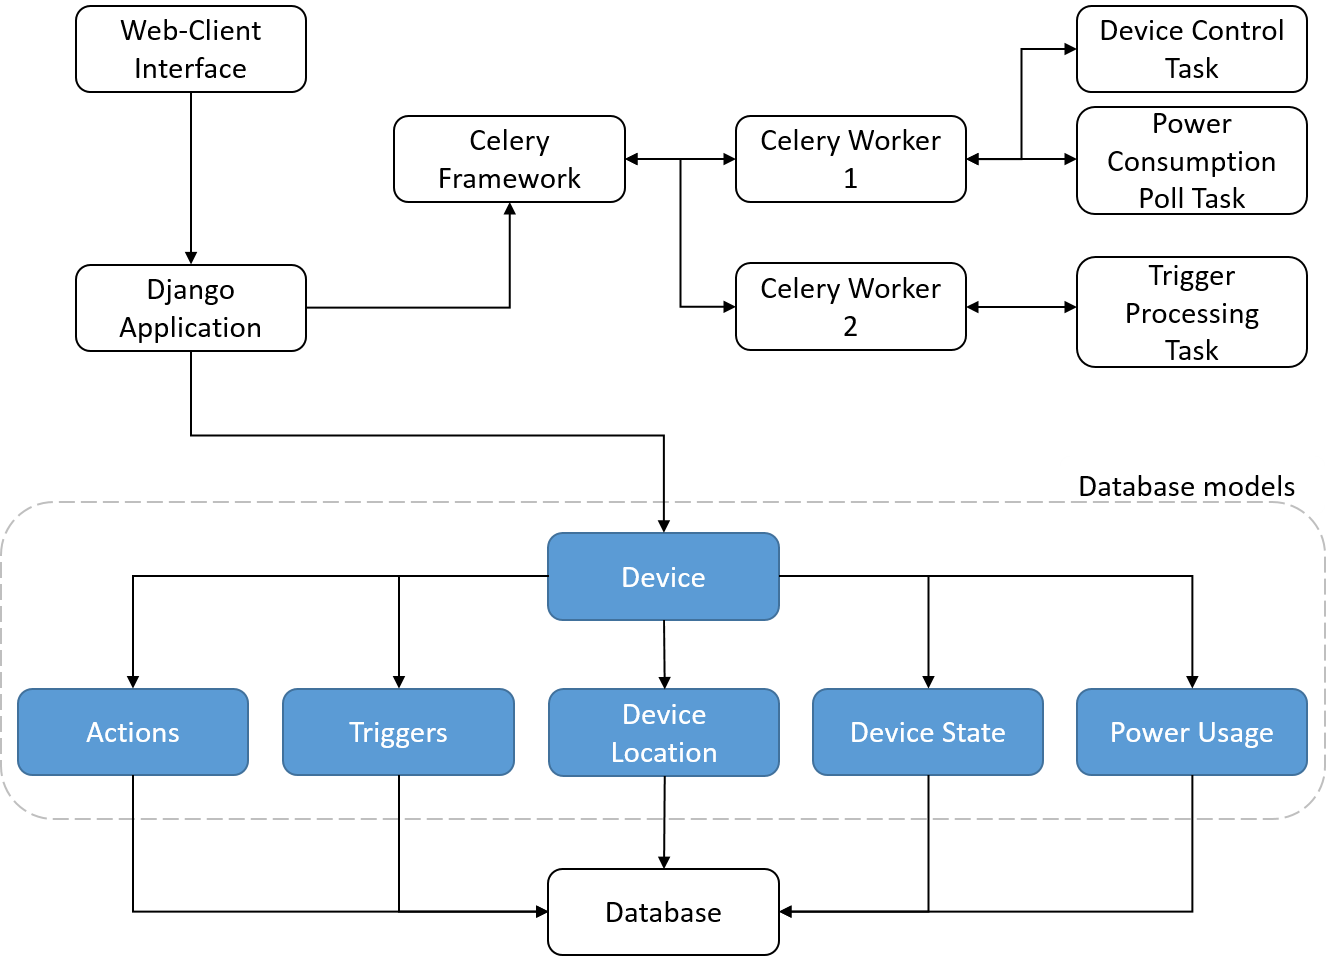
\includegraphics[width=\linewidth]{Sys_Overview}
		\caption{System architecture diagram}
		\label{fig:Sys_Overview}
	\end{figure}
	
	\subsubsection{Constraints:}
	\begin{itemize}
		\item The user interface must be accessible through a web browser
		\item All devices in the system require wireless connectivity
	\end{itemize}
	
	\subsubsection{Assumptions:}
	\begin{itemize}
		\item All of the IoT devices will be connected to the same LAN
		\item Only a small number of simultaneous users and devices will be connected at once
	\end{itemize}
	
	\subsection{Object Descriptions}
	\begin{itemize}
		\item \textbf{Django Application:} This section is the main application responsible for serving the front end and controlling the database interactions. It uses the Django framework in order to implement this functionality 
		\item \textbf{Database Models:} 
		\begin{itemize}
			\item \textit{Device Model:} This model represents a singe device. It keeps track of relevant device information, including name, IP address, location, and state. It is the core model of the database system. Two devices cannot have the same name and location attributes. Additionally, no two devices can have the same IP address. 
			\item \textit{Device Location:} This model represents the location in the household where a device can be found. A location can store many devices, but a device can only be in one location. 
			\item \textit{Device State:} This model represents the various power states that a device can be in. It is initially populated with the values "on" and "off," however the user still has the ability to add more depending on device capability. 
			\item \textit{Triggers:} This model represents the various triggers that the system can incorporate, namely, motion, temperature, and light. 
			It stores an input device ID, an output device ID, and a string of Python code which will provide the conditions for the trigger to fire as well as the action to apply.
			\item \textit{Actions:}  This model represents the various actions that can be taken by the system when a trigger is fired. 
			\item \textit{Power Usage:} This model represents the  cumulated power usage of the household devices. It accepts the time frame provided by the user in the front end and returns the total power consumption corresponding to that time specification.  
		\end{itemize}
		\item \textbf{Celery:} 
		This is an asynchronous task queuing framework that supports scheduling and real-time operation. The Django application uses Celery in order to manage long running tasks such as trigger monitoring as well as controlling and monitoring devices. Using the default RabbitMQ message broker, and the MQTT messaging protocol, Celery communicates with Internet of Things devices over the network. 
		\begin{itemize}
			\item \textit{Celery Worker 1:} This worker will handle tasks requested by the user, such as changing the device state, or polling a device for power usage data. 
			\item \textit{Celery Worker 2:} This worker will periodically execute the trigger processing task by fetching all the triggers from the database and executing those actions which correspond to the trigger that was flagged. 
		\end{itemize}
	\end{itemize}
	
	\subsection{Non-Functional Requirements}
	\subsubsection{Performance Requirements:}
	The smart home power system is an application and system that is designed for efficiency. This means that the application as well as the connecting household components need to respond quickly and in real time. 
	\\\\
	The application will most likely undergo several updates and changes for the user's benefit. The system is required to update on user command. Updates will include further improvements to the application as well as fixes for issues that arise in operation.
	
	\subsubsection{Safety Requirements:} 
	The application as well as the system components need to take certain safety concerns into account. 
	\\\\
	Due to the fact that the application is essentially controlling most of a home's appliances and electricity usage, it is important that it monitors everything it is controlling to prevent problems that may arise. The application needs to ensure that any device connected in the system does not reach a dangerous level of usage. In this case, the application should either switch off the device in question or notify the user that something is not functioning correctly and needs to be addressed. 
	
	\subsubsection{Security Requirements:}
	Due to the fact that the system controls a user's home, it therefore requires security considerations to be taken into account.
	\\\\
	The system needs to ensure that only the user has access to the application to prevent external parties gaining control of the connected components within a house. This can be done with a signup, login and authentication process. 
	The components within the house that the application connects with, need to be protected from external parties and therefore they must be explicitly authenticated. 
	
	\subsubsection{Software Quality Attributes:}
	The application is web based and needs to be user friendly. The functioning of the application needs to be simple so that no additional documentation or prior knowledge or experience is required. 
	
	\subsection{Supplementary Documentation}
	\subsubsection{Tools used to create diagrams:}
	\begin{itemize}
		\item UML diagrams: ArgoUML, http://argouml.tigris.org
	\end{itemize}
	
	\section{SPRINT PLANNING}
	
	The product backlog drawn up on 24 March 2016 is as shown below (ordered by priority):
	
	\begin{itemize}
		\item As a user I would like to be able to add/remove a device
		\begin{itemize}
			\item Create form to add new device
			\item Create list of devices which can be disabled/removed
		\end{itemize}
		\item As a user, I would like to be able to manually switch on and off appliances remotely
		\begin{itemize}
			\item Create page header menu
			\item Create sidebar and container
			\item Create page tabs
		\end{itemize}
		\item As a user I would like to view which devices are using power, and how much they are using
		\begin{itemize}
			\item Create dummy data on backend
			\item Create basic power usage graph for each device
		\end{itemize}
		\item As a user I would like to personalise various situations which will trigger an action
		\begin{itemize}
			\item Create list of different triggers 
			\item Create trigger settings page 
			\item Create form to choose triggers
		\end{itemize}
		\item As a user I need to choose which events should result in an immediate alert or notification on my system
		\begin{itemize}
			\item Logic to monitor status of different subsystems
			\item Configure how alert will be sent to user and connect accordingly
		\end{itemize}
		\item As a user it is convenient for me to be able to define webpage settings in order to enhance the power management system experience
		\item As a developer I want to be able to easily run the server using Docker
		\begin{itemize}
			\item Set up docker
			\item Configure docker to run server and database
		\end{itemize}
	\end{itemize}
	
	On this day, with two weeks remaining till project submission, a sprint planning meeting was held in order to discuss and plan the work to be performed in the first sprint which would have a timebox of one week. The screenshot below illustrates the items from the product backlog that were moved to the sprint backlog on this day. 
	
	\begin{figure}[H]
		\centering
		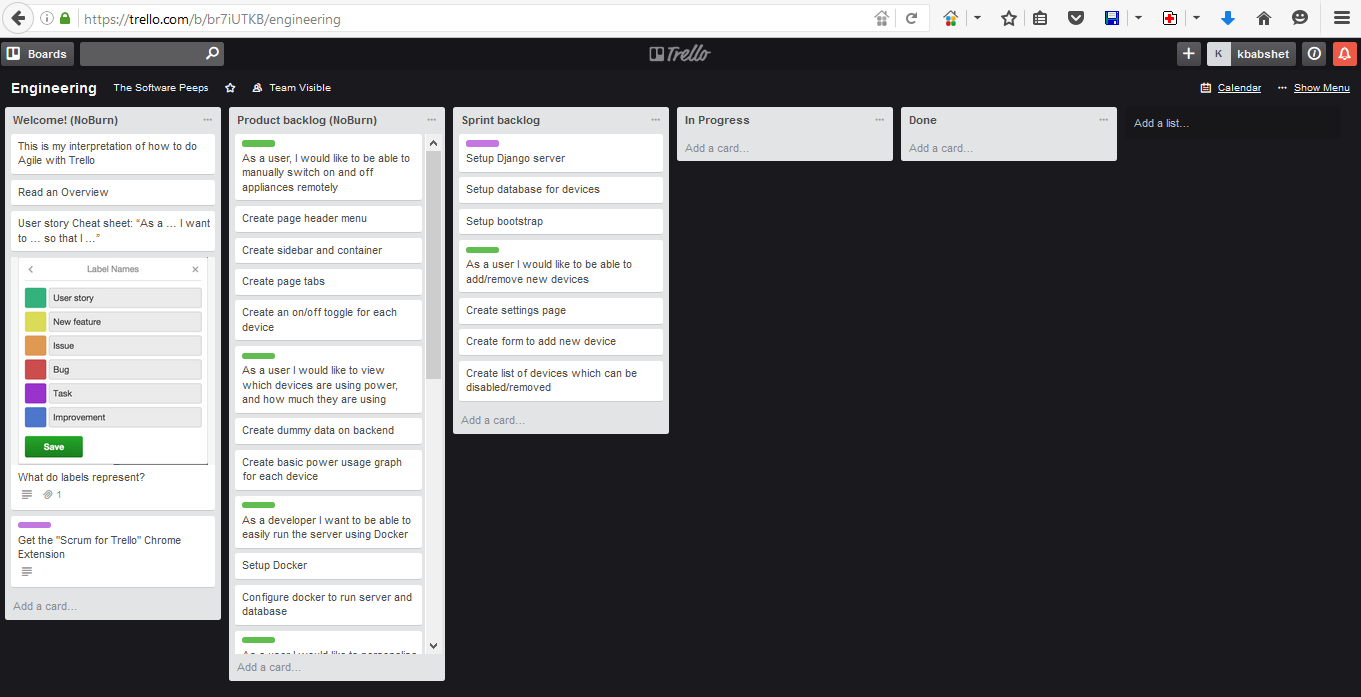
\includegraphics[width=\linewidth]{sprint_backlog_1}
		\caption{Screenshot of the Trello page drawn on the first day of the first sprint for the initial prototype implementation}
		\label{fig:sprint_backlog_1}
	\end{figure}
	
	After the first week, a second sprint planning was held for the following week-long sprint. The screenshot below illustrates the new items that were now moved to the next sprint backlog. 
	
	\begin{figure}[H]
		\centering
		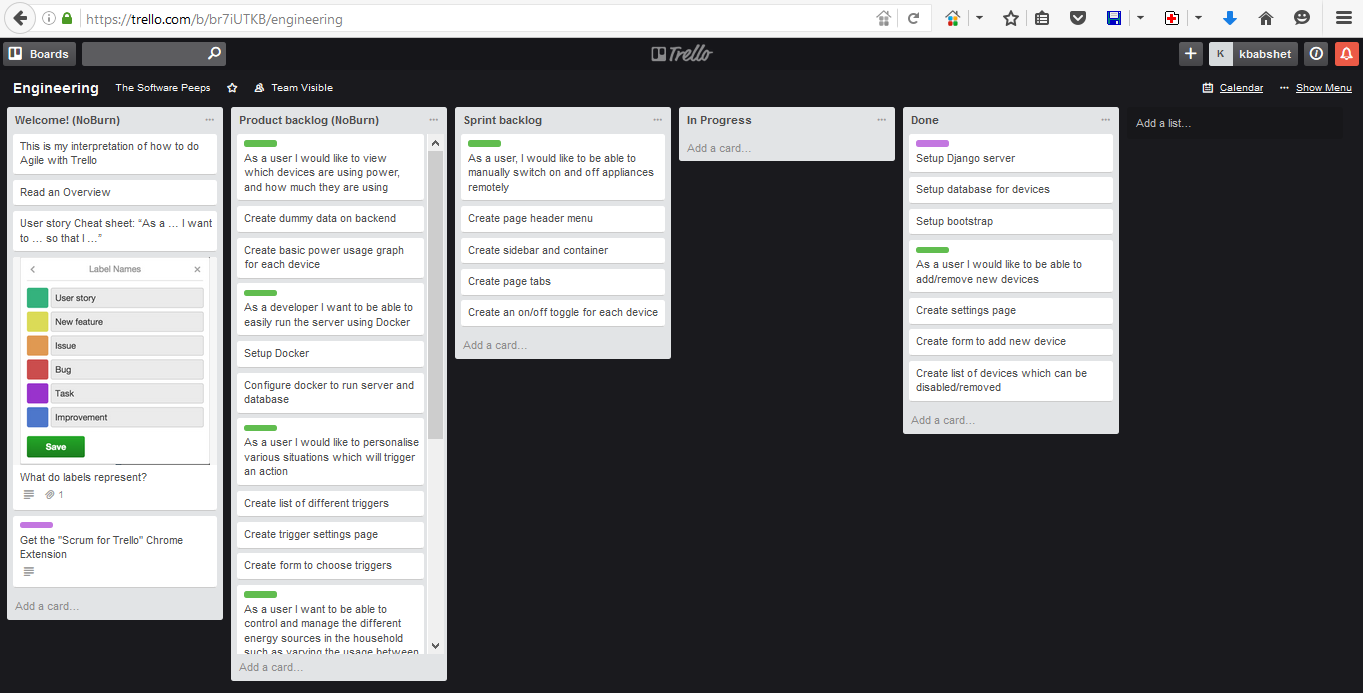
\includegraphics[width=\linewidth]{sprint_backlog_2}
		\caption{Screenshot of the Trello page drawn on the first day of the second sprint of the for the initial prototype implementation}
		\label{fig:sprint_backlog_2}
	\end{figure}
	
	\section{DESCRIPTION OF RELEVANT MODULES}
	Refer to the "Object Descriptions" (Section 3.4) within the Design Document for a presentation of the relevant modules implemented in the smart home power management system. 
	\section{SPRINT RETROSPECTIVE}

	%\newpage
	%\bibliographystyle{witseie}
	%\begin{thebibliography}{9}		
	%\end{thebibliography}
	
	%\newpage
	%\onecolumn
	%\section*{Appendix A}
	
	\newpage
	\pagebreak
	\bibliographystyle{IEEEtran}
	\bibliography{sample}
	
	%{\tiny \vfill \hfill \today \hspace{5mm} witseie-paper-2003.\TeX}
	
\end{document}

" vim: ts=4
" vim: tw=78
" vim: autoindent
" vim: shiftwidth=4
